% v2-acmtog-sample.tex, dated March 7 2012
% This is a sample file for ACM Transactions on Graphics
%
% Compilation using 'acmtog.cls' - version 1.2 (March 2012), Aptara Inc.
% (c) 2010 Association for Computing Machinery (ACM)
%
% Questions/Suggestions/Feedback should be addressed to => "acmtexsupport@aptaracorp.com".
% Users can also go through the FAQs available on the journal's submission webpage.
%
% Steps to compile: latex, bibtex, latex latex
%
% For tracking purposes => this is v1.2 - March 2012
\documentclass{acmtog} % V1.2

%\acmVolume{VV}
%\acmNumber{N}
%\acmYear{YYYY}
%\acmMonth{Month}
%\acmArticleNum{XXX}
%\acmdoi{10.1145/XXXXXXX.YYYYYYY}

\acmVolume{1}
\acmNumber{1}
\acmYear{2017}
\acmMonth{November}
\acmArticleNum{1}
\usepackage{float}
\usepackage{graphicx}
\usepackage{amsmath}
\usepackage{listings}
\usepackage{amssymb}


% Copyright
\setcopyright{rightsretained}


\begin{document}

\markboth{V. F. Pamplona et al.}{Photorealistic Models for Pupil Light Reflex and Iridal Pattern Deformation}

\title{Comparison between LTL and CTL } % title

\author{Qifeng Lin \\ 17214656}
% NOTE! Affiliations placed here should be for the institution where the
%       BULK of the research was done. If the author has gone to a new
%       institution, before publication, the (above) affiliation should NOT be changed.
%       The authors 'current' address may be given in the "Author's addresses:" block (below).
%       So for example, Mr. Fogarty, the bulk of the research was done at UIUC, and he is
%       currently affiliated with NASA.


\maketitle

    LTL is the abbreviation of Linear Temporal Logic, which can express some important properties of the system. It can give a LTL formula over the set of atomic propositions to guarantee the properties of the system. The LTL formula can be formed using following grammer:
    \begin{equation*}
      \varphi::=\text{true}|a|\varphi_1\wedge\varphi_2|\neg\varphi|\bigcirc\varphi|\varphi_2\text{U}\varphi_2
    \end{equation*}
    \begin{itemize}
      \item $a$ represents an atomic proposition.
      \item $\varphi_1\wedge\varphi_2$ means that both $\varphi_1$ and $\varphi_2$ should be satisfied at the same time.
      \item $\neg\varphi$ means that $\varphi$ should not occur.
      \item $\bigcirc\varphi$ means that the next state of the current state should satisfy $\varphi$
      \item $\varphi_2\text{U}\varphi_2$ means that holds at the current moment, if there is some future moment for which $\varphi_2$ holds and $\varphi_1$ holds at all moments until that future moment
    \end{itemize}
    
    It then can derive other operators as the following equations shows:
    \begin{equation*}
      \begin{aligned}
        \varphi_1\vee\varphi_2 & \overset{\text{def}}{=} \neg(\neg\varphi_1\wedge\neg\varphi_2) \\
        \varphi_1\rightarrow\varphi_2 & \overset{\text{def}}{=}\neg\varphi_1\vee\varphi_2\\
         \varphi\leftrightarrow\varphi_2 & \overset{\text{def}}{=}(  \varphi_1\rightarrow\varphi_2)\wedge(  \varphi_2\rightarrow\varphi_1)\\
         \varphi_1\otimes\varphi_2 & \overset{\text{def}}{=} (\varphi_1\wedge\neg\varphi_2)\vee(\varphi_2\wedge\neg\varphi_1)
      \end{aligned}
    \end{equation*}
    
    There are also two temporal combinators $\Diamond$ and $\Box$ which means "eventually" and "always" respectively. They can be derived from U operator.
    \begin{equation*}
        \begin{aligned}
        \Diamond\varphi & \overset{\text{def}}{=}\text{true U}\varphi\\
      \Box\varphi & \overset{\text{def}}{=}\neg\Diamond\neg\varphi
        \end{aligned}
    \end{equation*}
    
    By combining the temporal combinators $\Diamond$ and $\Box$ , we can acquire another temporal combinator:
    \begin{equation*}
      \begin{aligned}
        \Diamond\Box\varphi & \quad\text{"infinitely often $\varphi$"}\\
        \Box\Diamond\varphi & \quad\text{"eventually forever $\varphi$"}
      \end{aligned}
    \end{equation*}
    $\Diamond\Box\varphi$ means that at any moment $j$ there is a moment $i\geqslant j$ where a $\varphi$-state is visited. $ \Box\Diamond\varphi$ means that from some moment $j$ on, only $\varphi$-states are visited.
    
    By using operators given above, we can express the properties which the system should satisfy. However, we can see that using operators above, it can only verify executions that will not split off. And CTL can solve this problem.
    
    Compared with LTL, CTL adds quantifiers $\forall$ and $\exists$, which represents "all" and "there exists one". In this way, CTL can describe different paths.
    
    Take Fig.1 as an example.
    \begin{figure}[H]
      \centering
      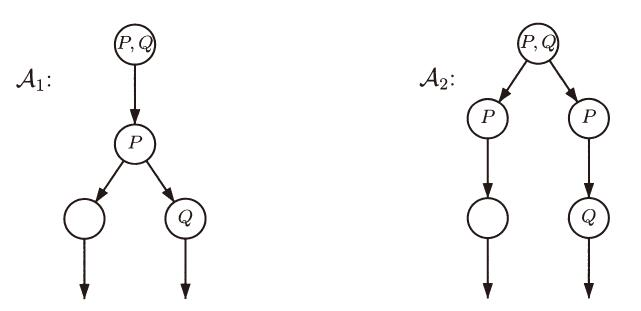
\includegraphics[width=3.0in]{5.jpg}
      \caption{Two automata, indistinguishable for LTL}
    \end{figure}
    
    In LTL, in initial state $q_0$ of $\mathcal{A}_1$, it will express as $\mathcal{A}_1,q_0\models\bigcirc P$. And in initial state $q_0'$ of $\mathcal{A}_2$, it also expresses as $\mathcal{A}_2,q_0'\models\bigcirc P$. However, the two automata are different with each other. Therefore, it cannot be applied under the condition. But CTL can solve the prolem. For $\mathcal{A}_1$, it will express as $\mathcal{A}_1,q_0\models\forall\bigcirc(\exists\bigcirc Q\wedge\exists\bigcirc\neg Q)$ whereas $\mathcal{A}_2,q_0'\nvDash\forall\bigcirc(\exists\bigcirc Q\wedge\exists\bigcirc\neg Q)$.
    
    CTL and LTL are two families of $\text{CTL}^*$ and they have their strength and weakness.




\end{document}
% End of v2-acmtog-sample.tex (March 2012) - Gerry Murray, ACM
